\documentclass[draft]{agujournal2019}
\usepackage{url} %this package should fix any errors with URLs in refs.
\usepackage{lineno}
\usepackage{booktabs}
\usepackage[inline]{trackchanges} %for better track changes. finalnew option will compile document with changes incorporated.
\usepackage{soul}
\linenumbers
%%%%%%%
% As of 2018 we recommend use of the TrackChanges package to mark revisions.
% The trackchanges package adds five new LaTeX commands:
%
%  \note[editor]{The note}
%  \annote[editor]{Text to annotate}{The note}
%  \add[editor]{Text to add}
%  \remove[editor]{Text to remove}
%  \change[editor]{Text to remove}{Text to add}
%
% complete documentation is here: http://trackchanges.sourceforge.net/
%%%%%%%

\draftfalse

%% Enter journal name below.
%% Choose from this list of Journals:
%
% JGR: Atmospheres
% JGR: Biogeosciences
% JGR: Earth Surface
% JGR: Oceans
% JGR: Planets
% JGR: Solid Earth
% JGR: Space Physics
% Global Biogeochemical Cycles
% Geophysical Research Letters
% Paleoceanography and Paleoclimatology
% Radio Science
% Reviews of Geophysics
% Tectonics
% Space Weather
% Water Resources Research
% Geochemistry, Geophysics, Geosystems
% Journal of Advances in Modeling Earth Systems (JAMES)
% Earth's Future
% Earth and Space Science
% Geohealth
%
% ie, \journalname{Water Resources Research}

\journalname{Journal of Advances in Modeling Earth Systems (JAMES)}


\begin{document}

%%%%%%%%%%%%%%%%%%%%%%%%%%%%%%%%%%%%%%%%%%%%%%%
%  TITLE
%
% (A title should be specific, informative, and brief. Use
% abbreviations only if they are defined in the abstract. Titles that
% start with general keywords then specific terms are optimized in
% searches)
%
%%%%%%%%%%%%%%%%%%%%%%%%%%%%%%%%%%%%%%%%%%%%%%%

% Example: \title{This is a test title}

\title{Escaping the simulation: using OSSE-trained mapping schemes on real altimetry}

\begin{keypoints}
\item We propose a simulation-based training approach for the neural mapping of real satellite-derived observations.
\item Simulation-trained neural schemes significantly outperform the operational mapping of real altimetry data for a Gulf Stream case-study.
%\item Learning from ocean simulations and simulated satellite altimetry data produces state-of-the-art mapping performance for real satellite-derived observations. 
\item More realistic simulation datasets improve the performance of the trained neural mapping both quantitatively and qualitatively. 
%\item Two ways to obtain more realistic synthetic data are increasing the resolution of the numerical simulation and model reanalysis.
\end{keypoints}

\begin{figure}[h!]
\small
\begin{center}
\setlength{\tabcolsep}{1pt}
\begin{tabular}{ccccc}
 &&
&\hspace{-30mm} 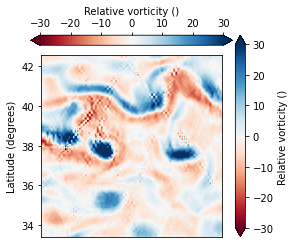
\includegraphics[trim={8mm 7cm 22mm 0},clip,width=5.0cm,height=1cm]{figures/plots/horizontal_cbar_vort.png} &\\
\hspace{0mm} &&
\hspace{-30mm} Training  
\hspace{3mm}  & 
 & 
\hspace{-30mm} Reconstruction \\

%\vspace{-2mm}
%%%%% ORCA025 %%%%%%%%

\hspace{-10mm}  1)&
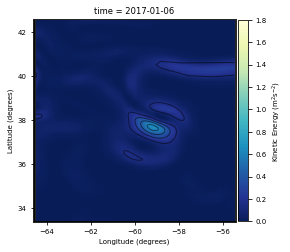
\includegraphics[trim={0 13mm 22mm 5mm},clip, width=3.60cm,height=3.2cm]{figures/plots/orca025_train_ke.png} &
 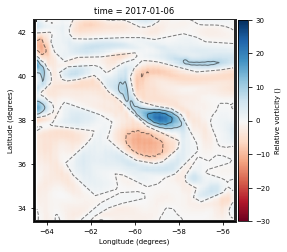
\includegraphics[trim={13mm 13mm 22mm 5mm},clip, width=3.2cm,height=3.2cm]{figures/plots/orca025_train_vort_r.png} &
 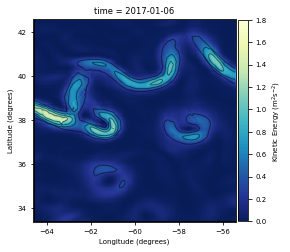
\includegraphics[trim={13mm 13mm 22mm 5mm},clip, width=3.2cm,height=3.2cm]{figures/plots/orca025_rec_ke.png} &
 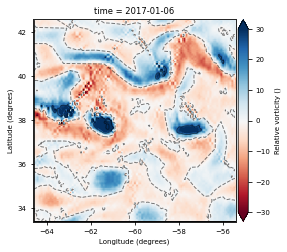
\includegraphics[trim={13mm 13mm 22mm 5mm},clip,width=3.2cm,height=3.2cm]{figures/plots/orca025_rec_vort_r.png} \\
%\vspace{3mm}
%%%%% GLORYS12-f %%%%%%%%
\hspace{-10mm} 2) &
 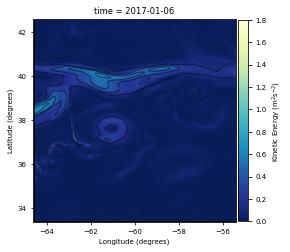
\includegraphics[trim={0 13mm 22mm 5mm},clip, width=3.60cm,height=3.2cm]{figures/plots/glorys12-f_train_ke.png} &
 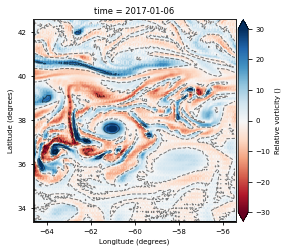
\includegraphics[trim={13mm 13mm 22mm 5mm},clip, width=3.2cm,height=3.2cm]{figures/plots/glorys12-f_train_vort_r.png} &
 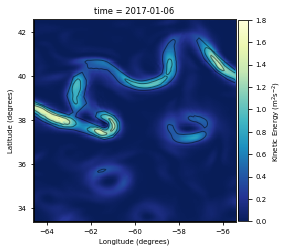
\includegraphics[trim={13mm 13mm 22mm 5mm},clip, width=3.2cm,height=3.2cm]{figures/plots/glorys12-f_rec_ke.png} &
 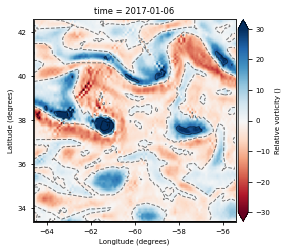
\includegraphics[trim={13mm 13mm 22mm 5mm},clip,width=3.2cm,height=3.2cm]{figures/plots/glorys12-f_rec_vort_r.png} \\
%\vspace{3mm}
%%%%% GLORYS12-f %%%%%%%%
\hspace{-10mm} 3) &
 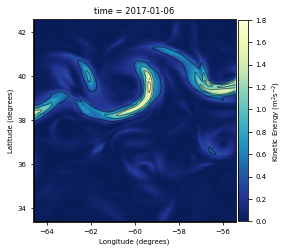
\includegraphics[trim={0 13mm 22mm 5mm},clip, width=3.60cm,height=3.2cm]{figures/plots/glorys12-r_train_ke.png} &
 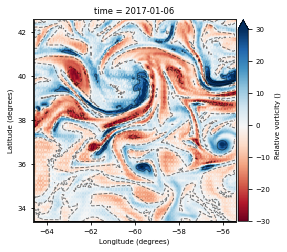
\includegraphics[trim={13mm 13mm 22mm 5mm},clip, width=3.2cm,height=3.2cm]{figures/plots/glorys12-r_train_vort_r.png} &
 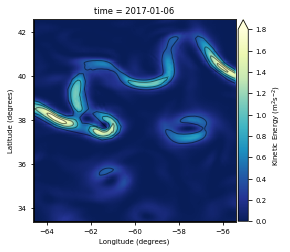
\includegraphics[trim={13mm 13mm 22mm 5mm},clip, width=3.2cm,height=3.2cm]{figures/plots/glorys12-r_rec_ke.png} &
 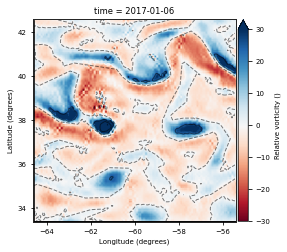
\includegraphics[trim={13mm 13mm 22mm 5mm},clip,width=3.2cm,height=3.2cm]{figures/plots/glorys12-r_rec_vort_r.png} \\
%%%%% NATL60 %%%%%%%%
\hspace{-10mm} 4) &
 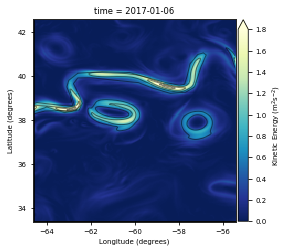
\includegraphics[trim={0 13mm 22mm 5mm},clip, width=3.60cm,height=3.2cm]{figures/plots/natl60_train_ke.png} &
 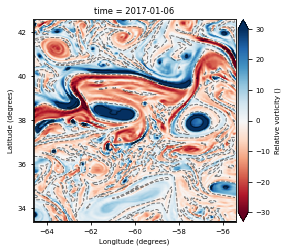
\includegraphics[trim={13mm 13mm 22mm 5mm},clip, width=3.2cm,height=3.2cm]{figures/plots/natl60_train_vort_r.png} &
 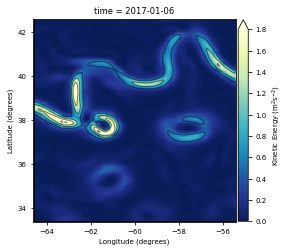
\includegraphics[trim={13mm 13mm 22mm 5mm},clip, width=3.2cm,height=3.2cm]{figures/plots/natl60_rec_ke.png} &
 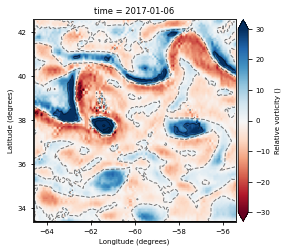
\includegraphics[trim={13mm 13mm 22mm 5mm},clip,width=3.2cm,height=3.2cm]{figures/plots/natl60_rec_vort_r.png} \\
%\vspace{3mm}
%%%%% eNATL60-t %%%%%%%%
\hspace{-10mm} 5) &
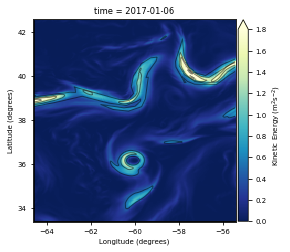
\includegraphics[trim={0 13mm 22mm 5mm},clip, width=3.60cm,height=3.2cm]{figures/plots/enatl60-t_train_ke.png} &
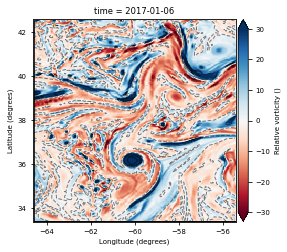
\includegraphics[trim={13mm 13mm 22mm 5mm},clip, width=3.2cm,height=3.2cm]{figures/plots/enatl60-t_train_vort_r.png} &
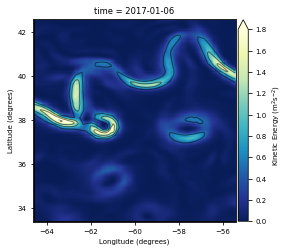
\includegraphics[trim={13mm 13mm 22mm 5mm},clip, width=3.2cm,height=3.2cm]{figures/plots/enatl60-t_rec_ke.png} &
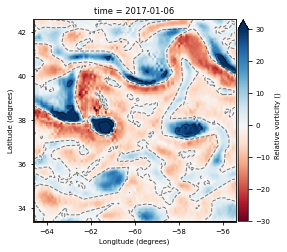
\includegraphics[trim={13mm 13mm 22mm 5mm},clip,width=3.2cm,height=3.2cm]{figures/plots/enatl60-t_rec_vort_r.png} \\
%\vspace{3mm}
%%%%% eNATL60-0 %%%%%%%%
\hspace{-10mm} 6) &
 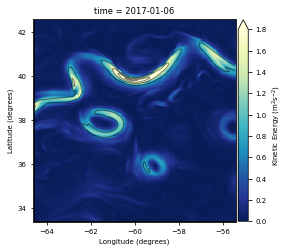
\includegraphics[trim={0 0 19mm 5mm},clip, width=3.60cm,height=3.4cm]{figures/plots/enatl60-0_train_ke.png} &
 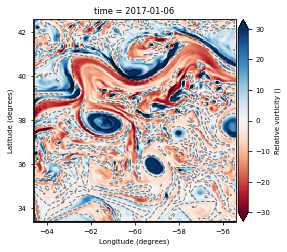
\includegraphics[trim={13mm 0 22mm 5mm},clip, width=3.2cm,height=3.4cm]{figures/plots/enatl60-0_train_vort_r.png} &
 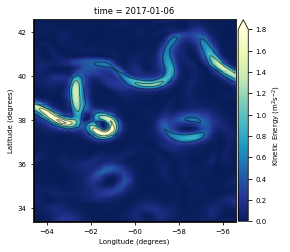
\includegraphics[trim={13mm 0 22mm 5mm},clip, width=3.2cm,height=3.4cm]{figures/plots/enatl60-0_rec_ke.png} &
 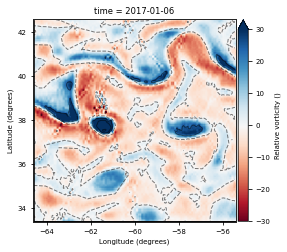
\includegraphics[trim={13mm 0 22mm 5mm},clip,width=3.2cm,height=3.4cm]{figures/plots/enatl60-0_rec_vort_r.png} \\
 \hspace{-15mm} &(a) & (b) & (c) & (d) \\
 &&
&\hspace{-30mm} 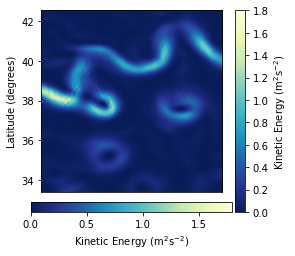
\includegraphics[trim={8mm 0 22mm 7cm},clip,width=4.5cm,height=1cm]{figures/plots/horizontal_cbar_ke_bottom.png} &\\
% \vspace{-2mm}

\end{tabular}
\vspace{-3mm}
% \caption{Row I - Isotrophic PSD. Row 2 - Isotrophic PSD Score}
\caption{
Kinetic energy ((a) and (b) and relative vorticity ((c) and (d)) of the training dataset ((a) and (c)) and the associated 4dVarNet reconstructions ((b) and (d)) at the 6th of January.
Each row shows the experiment using: 1) ORCA025, 2) GLORYS12-f, 3) GLORYS12-r, 4) NATL60, 5) eNATL60-t, eNATL60-0}
\vspace{-5mm}
\label{fig:maps}
\end{center}
\end{figure}

\section{Introduction}


% ML pour traitement de données satellite, bcp d'applications recentes 

% en particulier tache de gap-filling et cartoigraphie 

% un bon exemple altimétrie, methodes expertes et methodes methodes basées données. 

%--- [difficulté : suprenante, pas vraiment assez de données pour entrainer algo complexe (millions partame) [en fait non]]

% algo basé donnée : modele parametrique (calibration faible nombre de params : MIOST, DYNMOST), algo issue du DL (grnd nombre de param, NN expressif, peu d'hypothese)

% algo DL, besoin de bcp de données, en prqtique, peuvent entrainée sur données modeles. ex papier de SEATTLE. (emergence : modele numerique pour ca.) 

% question comment se fait le tranfert, sous quelle condition un lodele est-il bon poru entrainer algo pour tache donées reel. 

% Dans cet article, on demontre que modele peut marcher, cas particuler altimétrie, influence de la donnée d'entrée 

% le plan de l'artle, c'est ca 



\textbf{[Stake] : Large amount of data are observed from the ocean with important questions to be answered for climate understanding.} (...)

\subsection{Challenge}
Machine learning is a promising tool to fully benefit from the data but 


learning from observations presents many challenges due to gaps, noise and unobserved quantities. 

\subsection{Altimetry}
Satellite altimetry mapping is a good use case due to the high rate of missing data and to the fact that learning based methods have shown their potential in simulated setups raising the question of real world application.


\section{Background}

\subsection{SSH gridded products}


% la SSH, champ essentiel prou les ocean (ex : contrainte pour suysteme de predictiopn, reconstrutcion de coutrant pour SAR, ...)

% on l'utilise sou forme de produit grillée. ex DUACS delivré par coperniucus. 

% recent années dev de new algo : prior physique simple (BFN-QG, MIOST) ou pur data based. (4DVARNET)

% papier seatle : le meilleur algo basé donné (utilisant uniquement SSH), est un algo entrafinée sur données modele. 

Current SSH gridded products come from OGCM reanalysis or observation products made with minimal hypothesis like DUACS and BFN QG.

Learning based approaches have shown promise in simulated setups but the application to real data raises challenges.

\begin{itemize}
    \item MUSTI + ConvLSTM uses SST to reach SOTA
    \item ConvLSTM uses 10 years altimetry but drop in perf
\end{itemize}

We present a method to develop learning-based approaches for real altimetry tracks interpolation.

\subsection{Ocean Modeling and OSSE}
The use of ocean simulations has been crucial for gaining a deeper understanding of the earth system and predicting its behavior, while also serving as a valuable tool to test observation analysis methods. 

We introduce a  way to exploit those simulations to train machine learning models for real world purposes. 

\subsection{Transfer Learning and synthetic datasets}
In computer vision, it is a common practice to train models on datasets with verified ground truth when annotated data is scarce or unavailable,

\begin{itemize}
    \item annotated: Imagenet + transfer learning
    \item synthetic: flownet : syntel + flying chairs
\end{itemize}

We propose a similar approach in ocean science using numerical model outputs.

\subsection{Physics-aware deep-learning}
Recent works have found ways to combine ML methods with physical priors, however most of them have focused on simple physical models and it remains challenging to combine current OGCM with such methods.

We ask if training using an OGCM simulation is a valid way to combine the OGCM physics with deep-learning.

\section{Method: Simulation-based learning}

\subsection{Overview of the approach}
Simulation-based learning consists in simulating the ocean as well as the observing system in order to train an operator to perform on real observations.

\subsection{Synthetic SSH data}
We consider six synthetic dataset allowing to analyze the impact of three factors which are the numerical simulation resolution, observation data assimilation and explicit tide modeling in the numerical model.

\subsection{OSSE training setup}
We use different ocean simulations from the NEMO model and use the same simulated observing system to analyze the impact of the synthetic data used for training.  

\subsection{OSE evaluation setup}
The evaluation of our model is done using one year altimetry data of where one satellite is solely used for evaluating the reconstructed field.

\subsection{Neural Mapping Scheme}
The 4DVarNet model is considered which has been shown to outperform concurrent approaches when evaluated in an OSSE setup and is therefore a good candidate for testing the transferability to OSE setup.



\section{Results}
\subsection{It Works !!}
Simulation-based training outperforms approaches trained on real data as well as approaches with explicit dynamical priors.

\subsection{More realistic data means better reconstruction}
We highlight that learning from a more realistic simulation improves the performance metrics and produces less artefacts in the reconstruction. 


\subsection{No measurable impact of explicit tide modeling}
We discuss here the lack of measured impact of explicit tide motion in the ocean model and attribute it to the preprocessing (removal of barotropic tides in altimetry tracks and daily averaging) and evaluation (1D evaluation may not measure impact of internal tide) of the OSE setup.

\section{Discussion}
This study facilitated thanks to standardized training and evaluation setups of the datachallenges
Opportunities for new collaboration between ocean physicist, modelers and operational oceanographers
Ocean model simulation can be seen as foundation model training in deep learning, the outputs are the results of large computations can find many downstream applications
Ocean model simulation outputs could become seminal datasets on which general purpose foundation model could be train and then be finetuned on observation data for region and task specific purposes



\end{document}